\documentclass[prb,preprint]{revtex4-1} 
% The line above defines the type of LaTeX document.
% Note that AJP uses the same style as Phys. Rev. B (prb).

% The % character begins a comment, which continues to the end of the line.

\usepackage{amsmath}  % needed for \tfrac, \bmatrix, etc.
\usepackage{amsfonts} % needed for bold Greek, Fraktur, and blackboard bold
\usepackage{graphicx} % needed for figures

\begin{document}

% Be sure to use the \title, \author, \affiliation, and \abstract macros
% to format your title page.  Don't use lower-level macros to  manually
% adjust the fonts and centering.

\title{Double-Slit Experiment \LaTeX}
% In a long title you can use \\ to force a line break at a certain location.

\author{Yumeng Melody Cao}
\email{mcao@smith.edu} % optional
% If there were a second author at the same address, we would put another 
% \author{} statement here.  Don't combine multiple authors in a single
% \author statement.
\affiliation{Department of Physics, Smith College, Northampton, MA 01063}
% Please provide a full mailing address here.

\author{He Claudia Yun}
\email{hyun@smith.edu}
\affiliation{Department of Physics, Smith College, Northampton, MA 01063}

% See the REVTeX documentation for more examples of author and affiliation lists.

\date{\today}

%____________abstract____________________________________________

\begin{abstract}
In this experiment we use a laser of wavelength 670nm to re-perform Young's Double-Slit Experiment which demonstrates the wave nature of light. The observed interference pattern is fitted using Fraunhofer model with a detailed calculating of Chi-Squared as an indication of the goodness of the fit, and is found to be consistent with the theory.
%The interference pattern of the double and single-slit diffraction can be determined theoretically using Young's equation. In this experiment we use a laser of wavelength 670nm to test out this wave nature of light. The observed interference pattern is compared to that of the theoretical Fraunhofer model with a detailed calculation of Chi-Squared as an indication of the goodness of the fit. (...input conclusion and summary)
\end{abstract}

\begin{figure}[b]
\centering
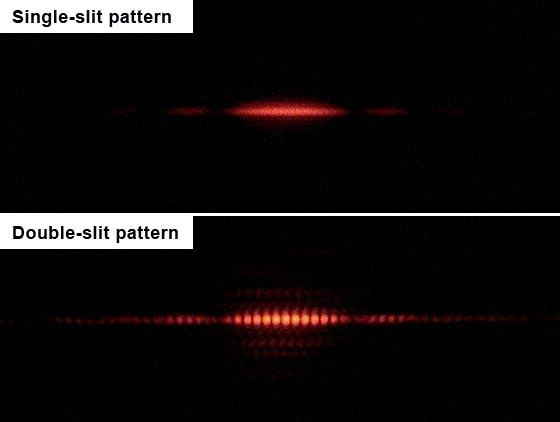
\includegraphics[width=4in]{image1.jpg}
\caption{Single and double-slit interference patterns \cite{wik}.}
\label{image}
\end{figure}

\maketitle % title page is now complete


%____________Introduction____________________________________________
\section{Introduction}
The double-slit experiment, also know known as the Young$^\prime$s experiment, explores the wave-like nature of light. It is important in this experiment for the two sources of light are coherent and have the same phase. Back in 1801, Thomas Young had difficulty with using common light sources, such as candles and lanterns, to be served as coherent sources of light. Thus instead, Young performed the experiment by filtering sunlight through a pinhole in a window shutter split by a piece of card and projecting it horizontally across the room. Light waves from either side of the card coming through the pinhole can be thus considered coherent sources and the interference pattern was then projected onto a screen from which the wavelength of the light source could be determined using Young$^\prime$s Equation: $$\lambda=\frac{y*d}{m*L}$$

Today, we can do the experiment by using the TWS apparatus that includes a monochromatic laser beam at one end (with a wavelength of 670 nm) passing through a double slit all encapsulated in a tightly sealed u-channel. Adjusting the micrometer attached to the detector-slit allows you to gather information regarding the interference pattern that is projected to a photodiode at the other end of the u-channel.

%____________Experiment____________________________________________
\section{Experiment}
In this experiment, the apparatus is set up as shown in Fig. \ref{dia}. After precise alignment of the laser, the double-slit, the slit-blocker, and the detector-slit, the photodiode is connected to a multimeter which is ultimately connected to the computer. LabView is used to collect data first for the double-slit experiment and for the single-slit experiment.

\begin{figure}[h!]
\centering
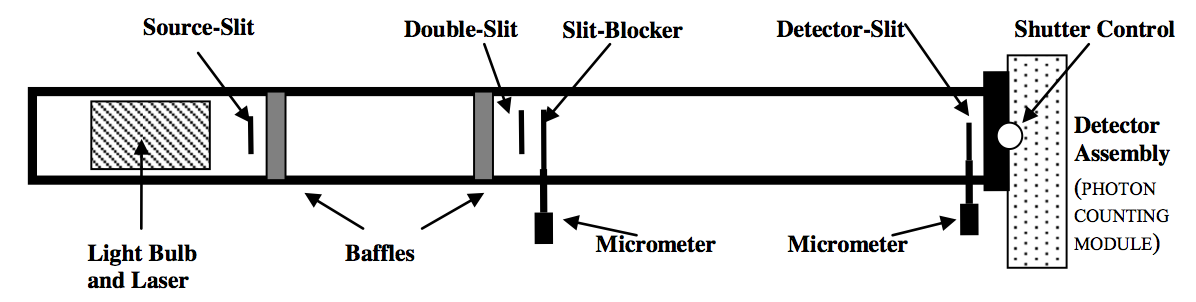
\includegraphics[width=7in]{dia}
\caption{Schematic of TWS apparatus - not to scale \cite{dia}.}
\label{dia}
\end{figure}
All parts are carefully aligned and key positions of the slit-blocker are recorded, so that light from one or two slits could be blocked and form both double-slit and single-slit interference patterns. The shutter at the end of the U-channel was kept closed, because only the photodiode on the surface of the shutter is used. After the preparation work, the double-slit experiment is first performed. A double-slit of slit width approximately 0.1 mm and slit separation 0.406 mm is used.

The slit-blocker is set at the position where light from both slits are allowed to pass, and the detector-slit is set at the position of the central maximum. The photodiode outputs a voltage that is proportional to the intensity of the laser beam.

By changing the position of the detector-slit, intensity of the laser light is recorded by LabView as a function of location. Then the experiment is repeated for single-slit when the slit-blocker blocks light from one of the two slits.
%____________Results____________________________________________
\section{Results}

Double slit intensity under Fraunhofer conditions: $$I=I_0 sinc^2( \frac{\pi a}{\lambda} sin \theta)  cos^2(\frac{\pi d}{\lambda} sin \theta)$$

\begin{figure}[h!]
\centering
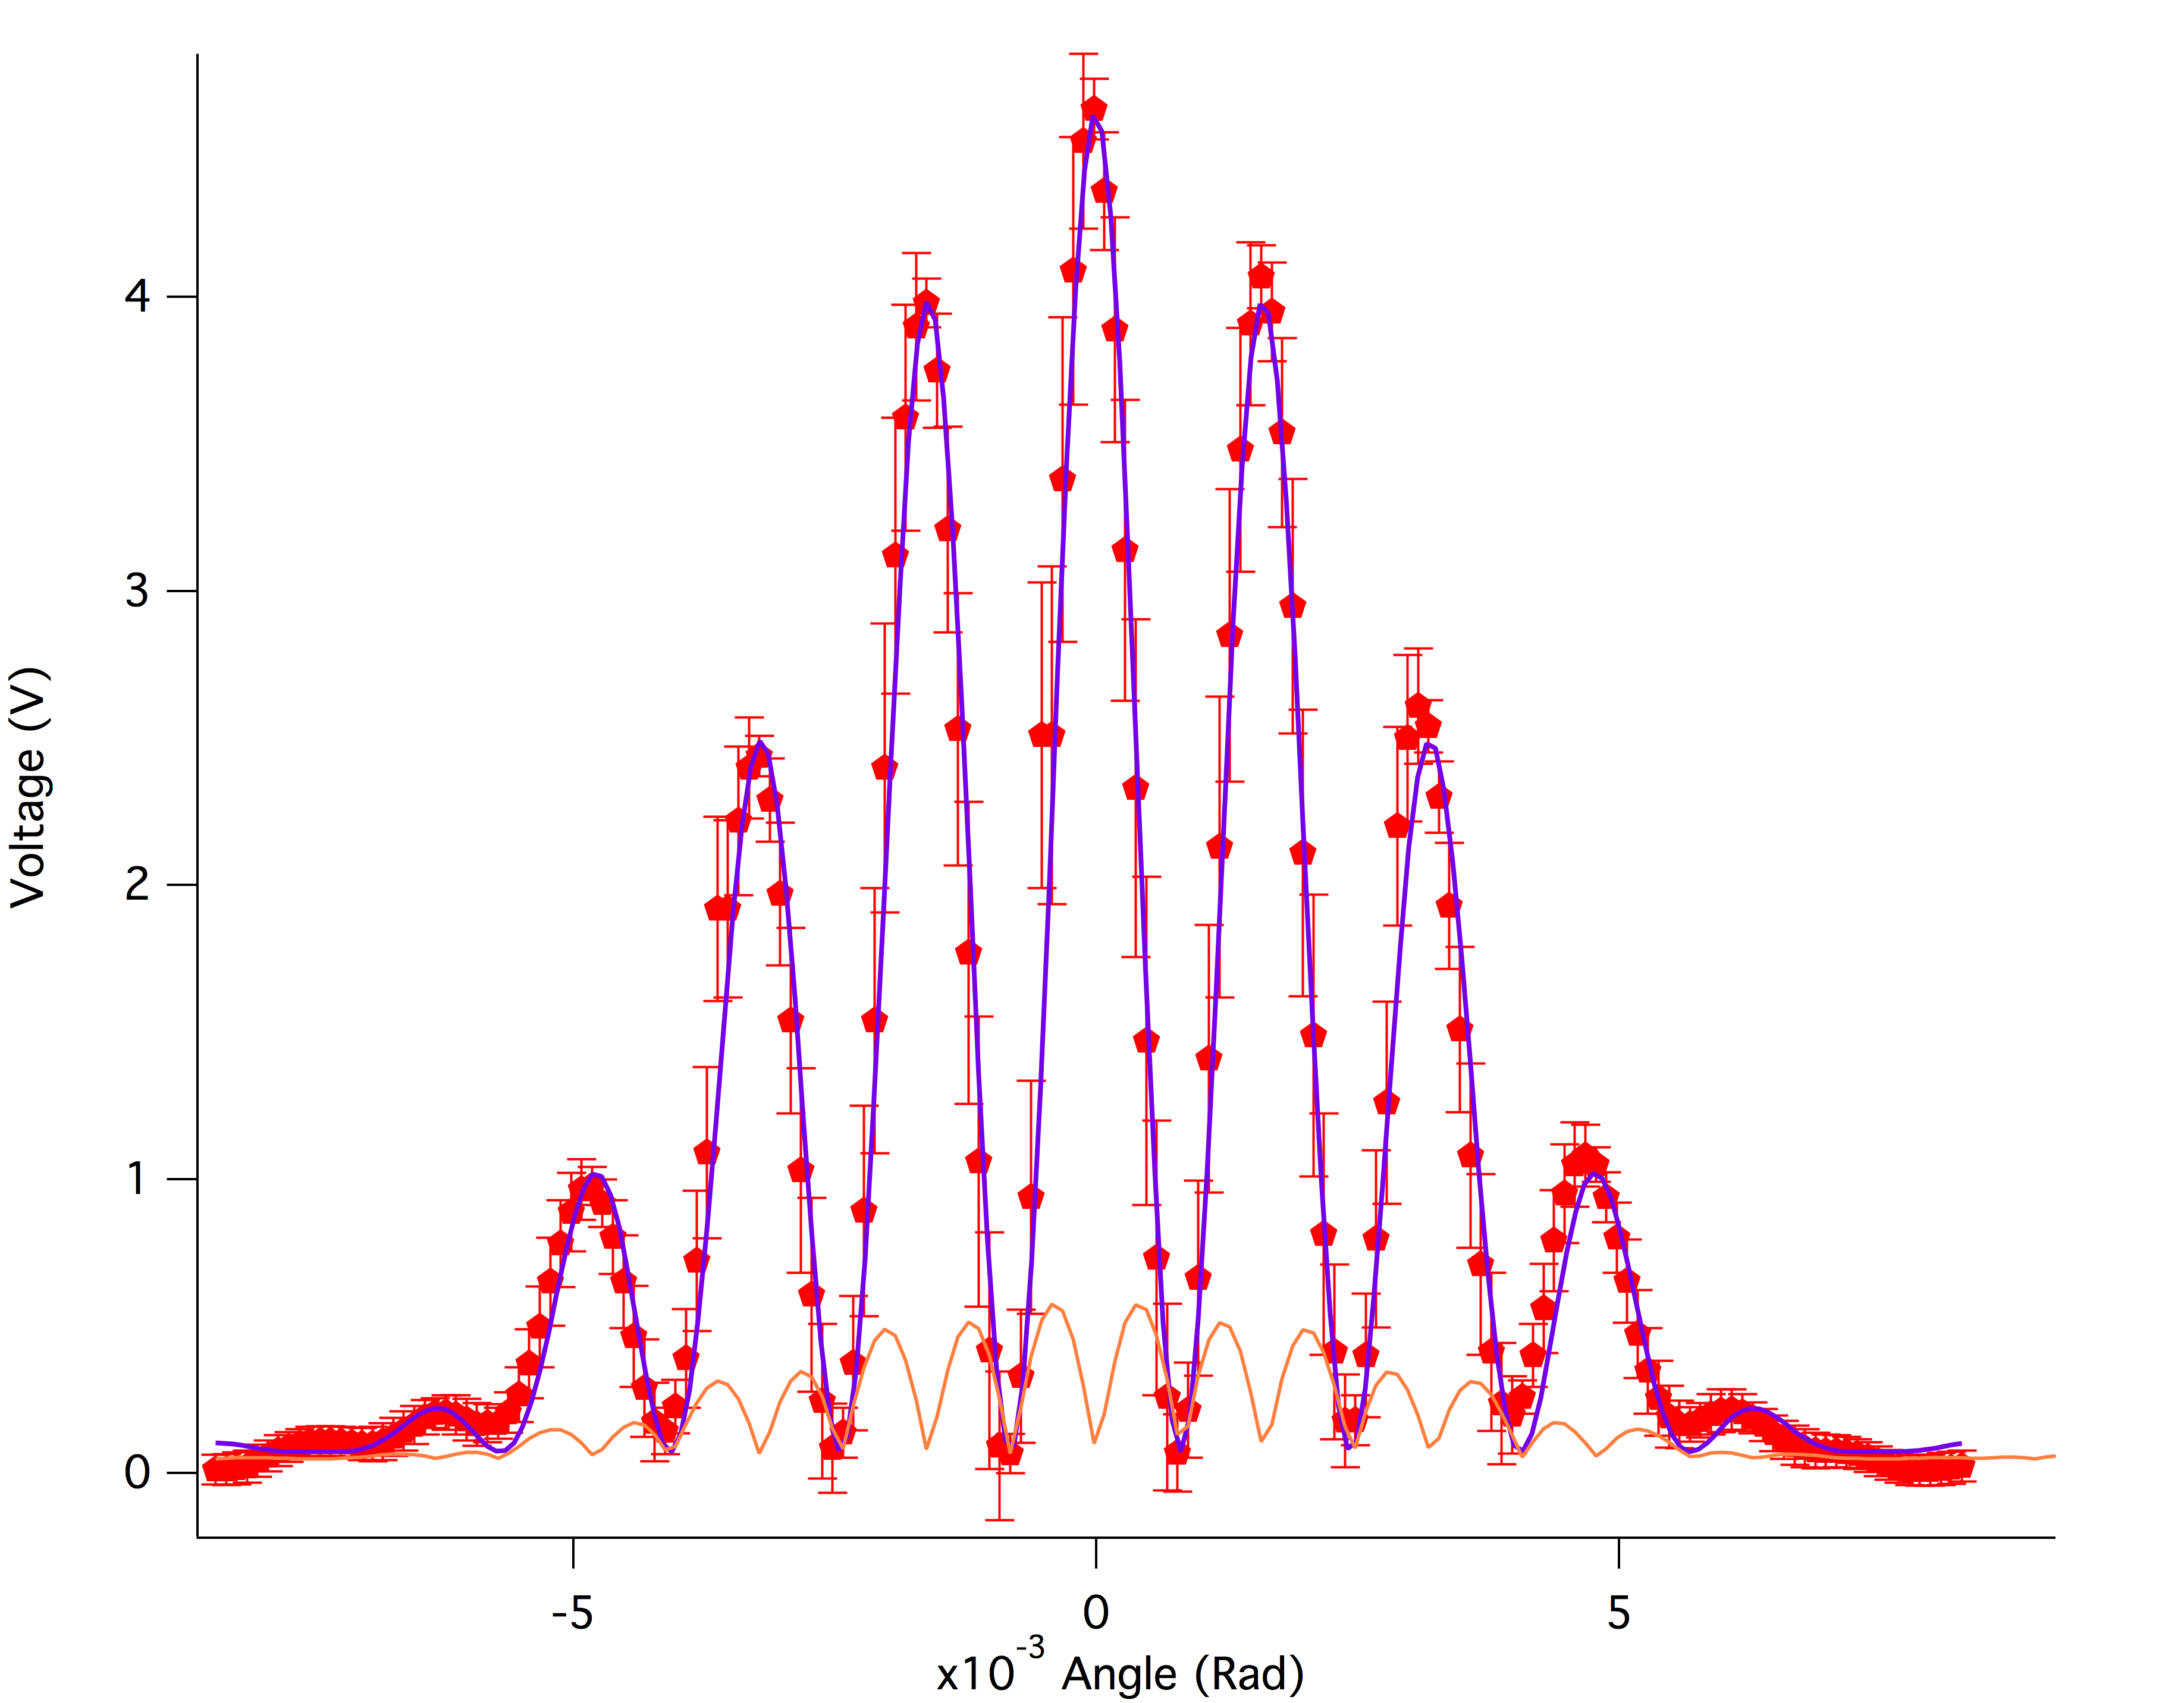
\includegraphics[width=7in]{double}
\caption{Plot of double slit interference.}
\label{double}
\end{figure}

Single slit under Fraunhofer conditions: $$I=I_0 sinc^2 (\frac{\pi a}{\lambda} sin\theta)$$

\begin{figure}[h!]
\centering
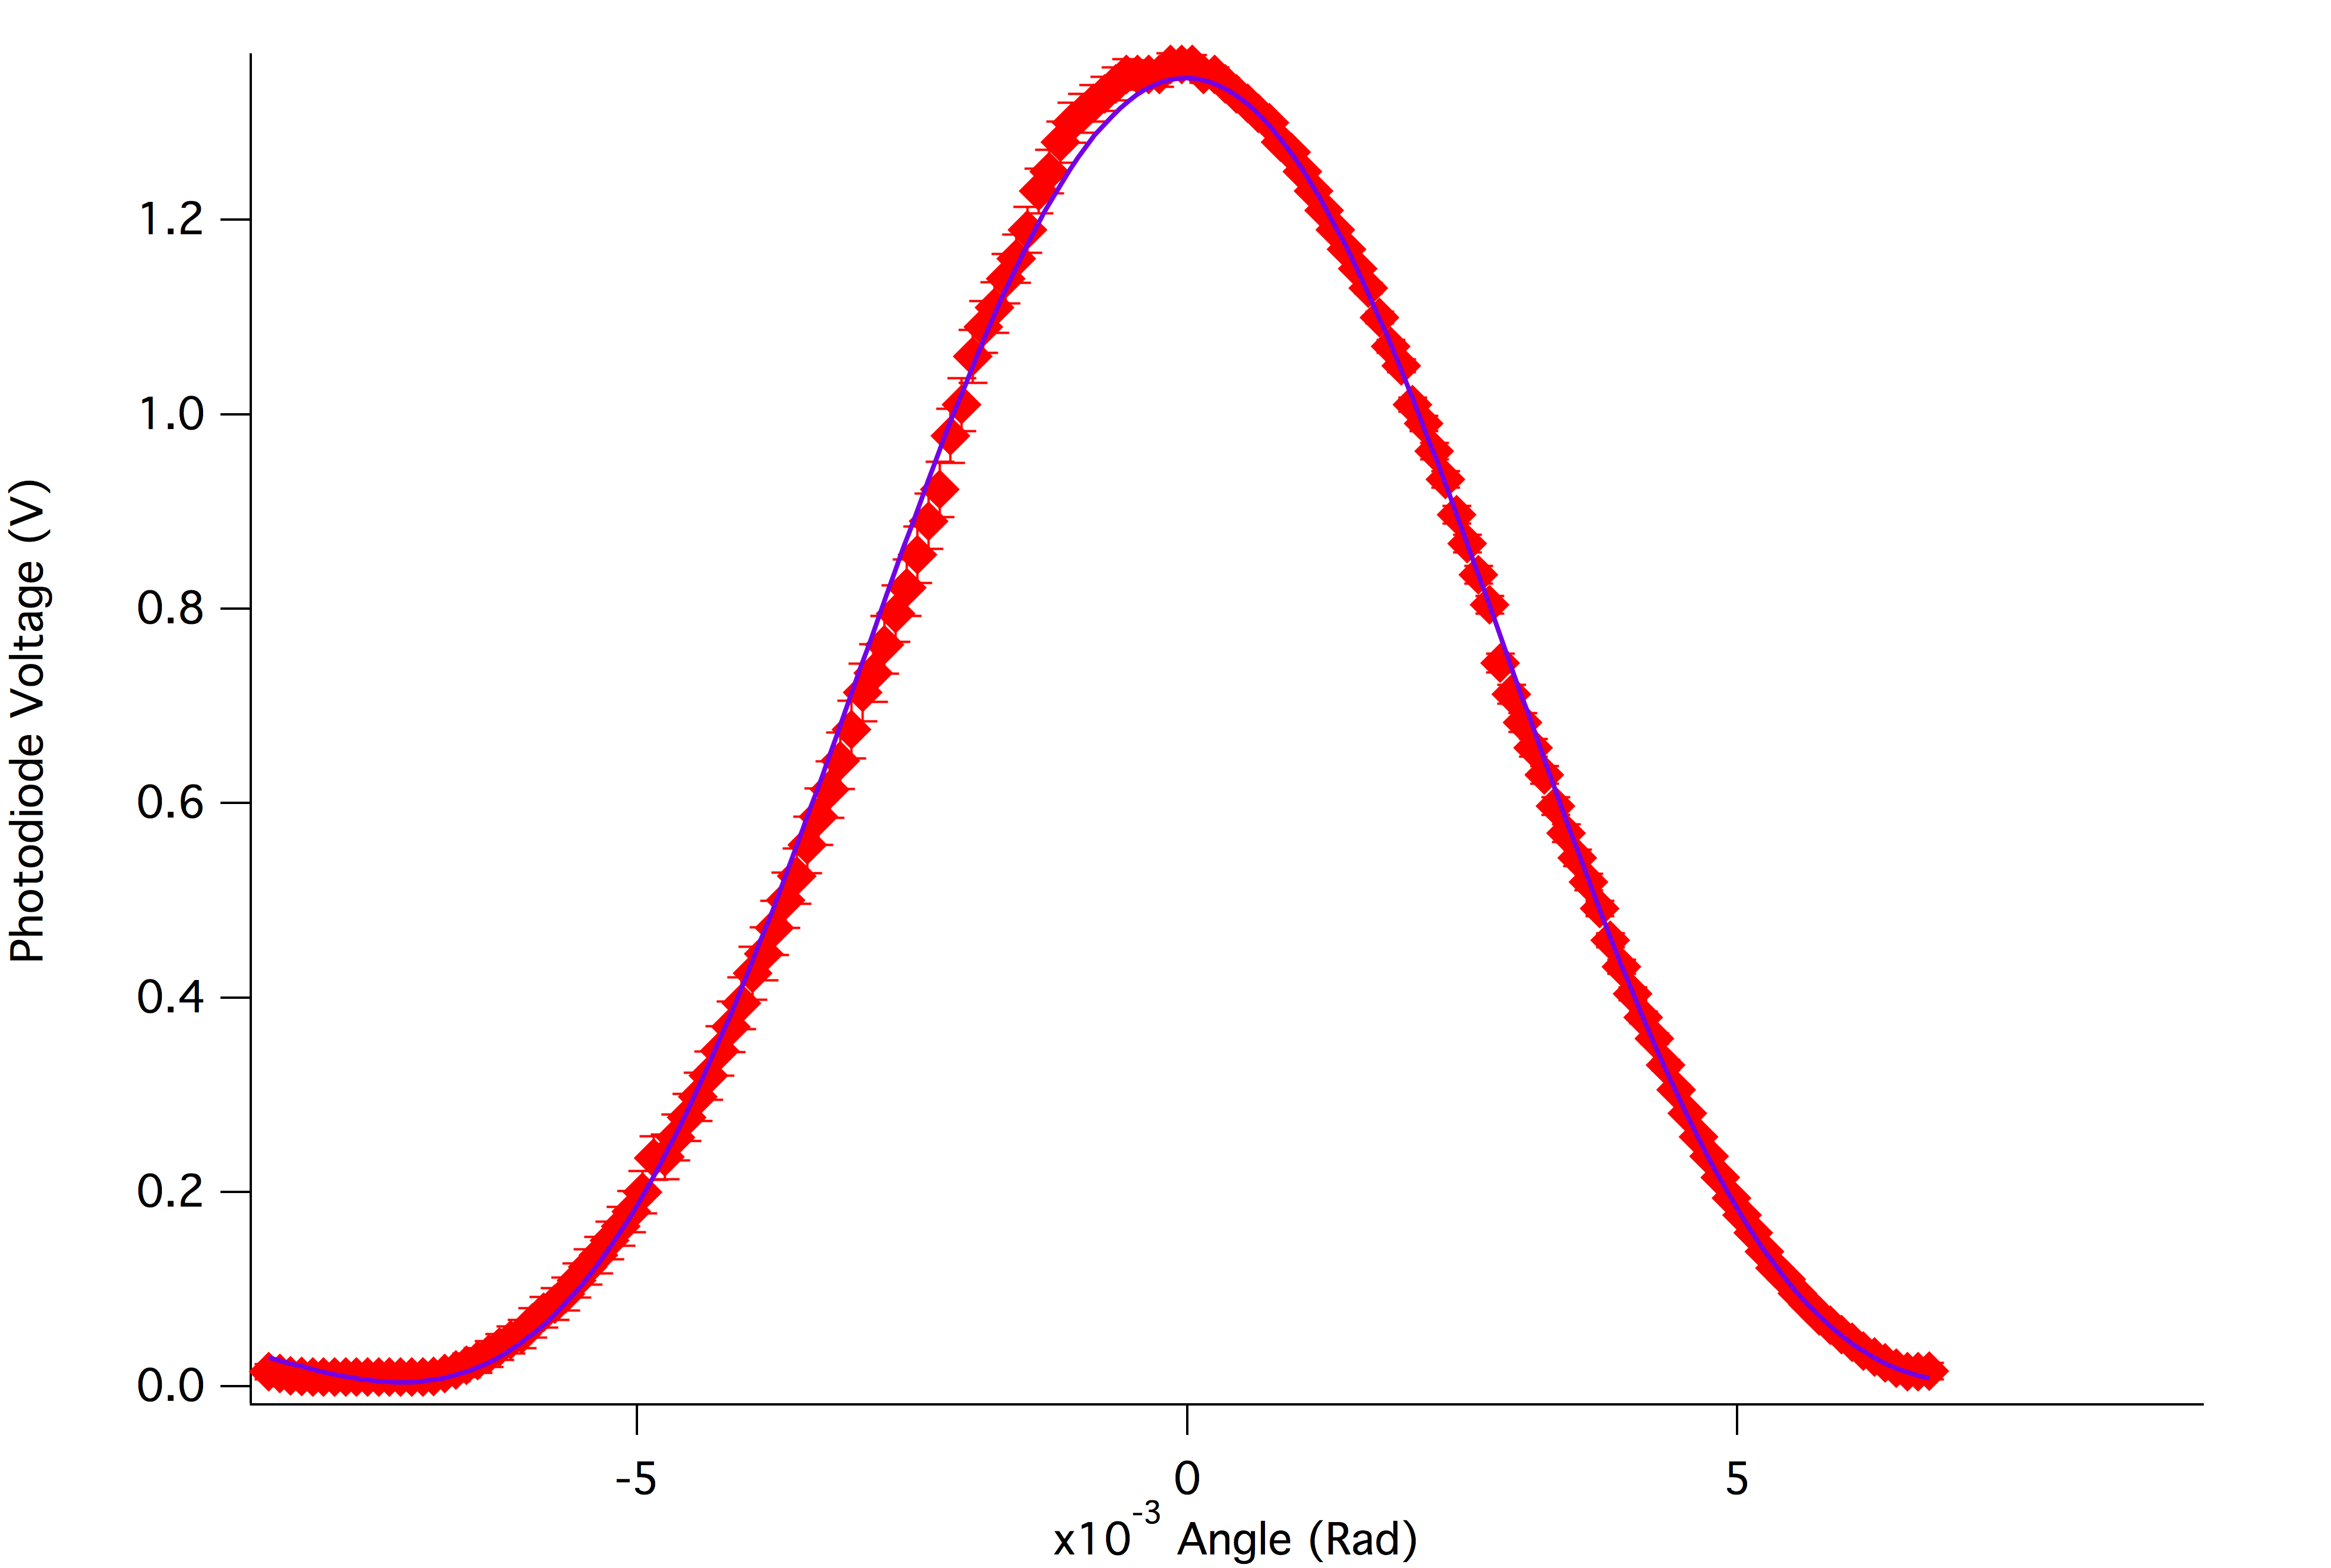
\includegraphics[width=7in]{single}
\caption{Plot of single slit interference.}
\label{single}
\end{figure}


%____________Discussion____________________________________________
\section{Discussion}


%____________Conclusion____________________________________________
\section{Conclusion}


\section{Figures}

\LaTeX\ can import figures via the \verb/\includegraphics/ macro.
For AJP, you should embed this in the \texttt{figure} environment, which 
can place the figure in various locations.  This environment also lets 
you add a caption (which AJP requires) and an optional label for referring 
to the figure from elsewhere.  See Fig.~\ref{gasbulbdata} for an example.



\section{Tables}

\begin{table}[h!]
\centering
\caption{Double slit data}
\begin{ruledtabular}
%\begin{tabular}{l c c c c p{5cm}}
\begin{tabular}{l c c}
% The codes above determine the horizontal alignment in each column.
% Options are l (left), r (right), c (centered), and p (paragraph).
% The p option allows an entry to be broken into multiple lines, and
% therefore requires a width specification, in this case 5 centimeters.
Name & Symbol & Value\\
\hline
Slit Separation & d & 0.016 in \\

\end{tabular}
\end{ruledtabular}
\label{data}
\end{table}


\begin{acknowledgments}

We gratefully acknowledge Harvey Gould and Jan Tobochnik, who created an earlier 
AJP \LaTeX\ sample article that inspired this one.  This work was supported by the 
American Association of Physics Teachers.

\end{acknowledgments}


\begin{thebibliography}{99}
% The numeral (here 99) in curly braces is nominally the number of entries in
% the bibliography. It's supposed to affect the amount of space around the
% numerical labels, so only the number of digits should matter--and even that
% seems to make no discernible difference.

\bibitem{wik} \LaTeX\ Double Slit Experiment, \url{<http://upload.wikimedia.org/wikipedia/commons/c/c2/Single_slit_and_double_slit2.jpg
/>}.

\bibitem{dia} \LaTeX\ TeachSpin Instructions Manual,\textit{Two-Slit interference, One Photon at a Time (TWS1-B), Pulse Counter/Interval Timer (PCIT1)}, 6/2013.

\bibitem{latexsite} \LaTeX\ Project Web Site, \url{<http://www.latex-project.org/>}.

\bibitem{wikibook} \textit{\LaTeX} (Wikibook), \url{<http://en.wikibooks.org/wiki/LaTeX/>}.

\bibitem{latexbook}Helmut Kopka and Patrick W. Daly, \textit{A Guide to
\LaTeX}, 4th edition (Addison-Wesley, Boston, 2004).

\bibitem{revtex} REV\TeX\ 4 Home Page, \url{<https://authors.aps.org/revtex4/>}.

\bibitem{cloudLaTeX} On the other hand, you can avoid the installation process
entirely by using a cloud-based \LaTeX\ processor such as ShareLaTeX,
\url{<https://www.sharelatex.com/>}, or write\LaTeX, \url{<https://www.writelatex.com/>}.

\bibitem{nevermindlogic} In typography, aesthetics often takes precedence over logic.

\bibitem{FontEncodingComment} Please don't try to handle foreign characters 
and accents with the \texttt{inputenc} and \texttt{fontenc} packages, which 
are incompatible with AJP's editing process.

\bibitem{wikimathpage} See the Mathematics chapter of Ref.~\onlinecite{wikibook}
for an excellent overview of math symbols and equations, with examples.

\bibitem{labelnames} Thinking up a good label name takes a moment, but 
it's worth the trouble; we strongly advise against using labels like 
\texttt{eq2}, which become extremely confusing after you decide to add 
another equation before Eq.~(\ref{deriv}).

\bibitem{footnotes} You need to process a file twice to get the counters correct.

\bibitem{mermin} N. David Mermin, ``What's wrong with these equations?,'' 
Phys. Today \textbf{42} (10), 9--11 (1989).  
% Note that the issue number (10) in this citation is required, because
% each issue of Physics Today starts over with page 1.  Also note the use of
% an en-dash (--), not a hyphen (-), for the page range.

\bibitem{editorsite} American Journal of Physics Editor's Web Site, 
\url{<http://ajp.dickinson.edu>}.

\bibitem{feynman} Richard P. Feynman, Robert B. Leighton, and Matthew Sands, 
\textit{The Feynman Lectures on Physics, Vol.\ 1} (Addison-Wesley, 1964), p.~3-10.
% Note that this book is paginated by chapter; "3-10" is a single page reference
% that uses a hyphen, not a range of pages that would us an en-dash (--).

\bibitem{noBIBTeX} Many \LaTeX\ users manage their bibliographic data with 
a tool called BIB\TeX.  Unfortunately, AJP cannot accept BIB\TeX\ files; all 
bibliographic references must be incorporated into the manuscript file
as shown here, at least when you send an editable file for production.

\bibitem{dyson} Freeman J. Dyson, ``Feynman's proof of the Maxwell equations,''
Am. J. Phys. \textbf{58} (3), 209--211.  
% The issue number (3) in this citation is optional, because AJP's pagination 
% is by volume.

\bibitem{examplevolume} M. R. Flannery, ``Elastic scattering,'' in 
\textit{Atomic, Molecular, and Optical Physics Handbook}, edited by
G. W. F. Drake (AIP Press, New York, 1996), p.~520.

\bibitem{AIPstylemanual} \textit{AIP Style Manual}, 4th edition (American 
Institute of Physics, New York, 1990). Available online at 
\url{<http://www.aip.org/pubservs/style/4thed/toc.html>}. Although parts of 
it have been made out of date by advancing technology, most of this manual 
is still as useful as ever. Just be sure to follow AJP's specific rules
whenever they conflict with those in the manual.

\end{thebibliography}

% If your manuscript is conditionally accepted, the editors will ask you to
% submit your editable LaTeX source file.  Before doing so, you should move
% all tables and figure captions to the end, as shown below.  Tables come 
% first, followed by figure captions (with figure inclusions commented-out).
% Figures should be submitted as separate files, collected with the
% LaTeX file into a single .zip archive.

%\newpage   % Start a new page for tables

%\begin{table}[h!]
%\centering
%\caption{Elementary bosons}
%\begin{ruledtabular}
%\begin{tabular}{l c c c c p{5cm}}
%Name & Symbol & Mass (GeV/$c^2$) & Spin & Discovered & Interacts with \\
%\hline
%Photon & $\gamma$ & \ \ 0 & 1 & 1905 & Electrically charged particles \\
%Gluons & $g$ & \ \ 0 & 1 & 1978 & Strongly interacting particles (quarks and gluons) \\
%Weak charged bosons & $W^\pm$ & \ 82 & 1 & 1983 & Quarks, leptons, $W^\pm$, $Z^0$, $\gamma$ \\
%Weak neutral boson & $Z^0$ & \ 91 & 1 & 1983 & Quarks, leptons, $W^\pm$, $Z^0$ \\
%Higgs boson & $H$ & 126 & 0 & 2012 & Massive particles (according to theory) \\
%\end{tabular}
%\end{ruledtabular}
%\label{bosons}
%\end{table}

%\newpage   % Start a new page for figure captions

%\section*{Figure captions}

%\begin{figure}[h!]
%\centering
%\includegraphics{GasBulbData.eps}   % This line stays commented-out
%\caption{Pressure as a function of temperature for a fixed volume of air.  
%The three data sets are for three different amounts of air in the container. 
%For an ideal gas, the pressure would go to zero at $-273^\circ$C.  (Notice
%that this is a vector graphic, so it can be viewed at any scale without
%seeing pixels.)}

%\label{gasbulbdata}
%\end{figure}

%\begin{figure}[h!]
%\centering
%\includegraphics[width=5in]{ThreeSunsets.jpg}   % This line stays commented-out
%\caption{Three overlaid sequences of photos of the setting sun, taken
%near the December solstice (left), September equinox (center), and
%June solstice (right), all from the same location at 41$^\circ$ north
%latitude. The time interval between images in each sequence is approximately
%four minutes.}
%\label{sunsets}
%\end{figure}

\end{document}
